\subsection{Subjective Evaluation}~\label{subjective}

In the preceding section, it was observed that the methods yielded diverse outcomes when tasked with a broad prompt, such as creating a `robot made of plants'. The text-to-3D methods faced challenges in initially generating an detailed object, a stark contrast to the image-to-3D methods that benefited from having a reference image, offering some directional guidance and hence a slight advantage. To establish a more leveled playing field for the various methods, the next prompt chosen for testing was \textbf{``a high-quality rendering of a Playmobil firefighter''}. Playmobil figures are known for their uniform base structures, differing primarily in clothing or texture. This prompt was therefore selected to assess whether a method could accurately capture the fundamental structure dictated by the prompt. The outcomes of each method, applied to this specific prompt, are illustrated in Figure~\ref{fig:resultPlaymobil}. 

\begin{figure}[ht]
    \centering
    \small
    \begin{subfigure}[b]{0.18\textwidth}
        \centering
        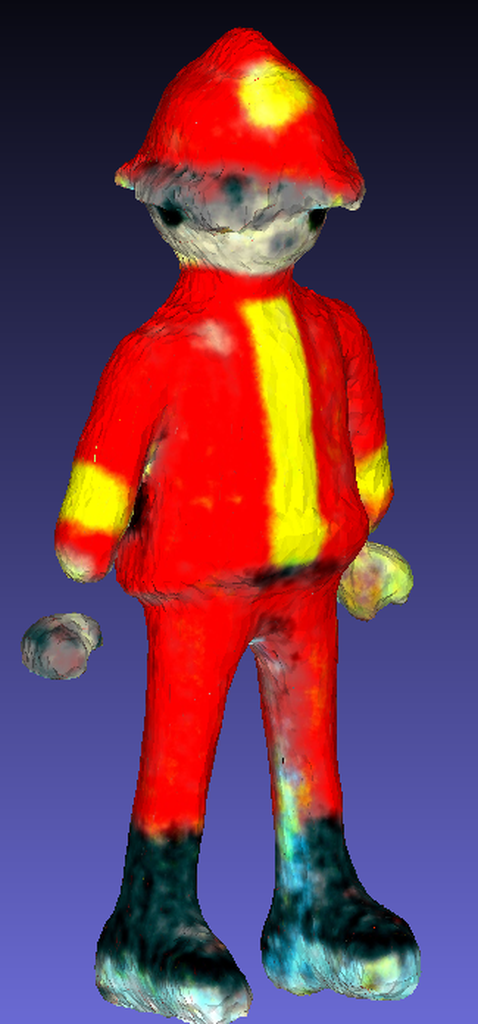
\includegraphics[width=\textwidth]{figures/subjective/dreamfusion_playmobil_result_resize.png}
        \caption{DreamFusion}
    \end{subfigure}
    \begin{subfigure}[b]{0.179\textwidth}
        \centering
        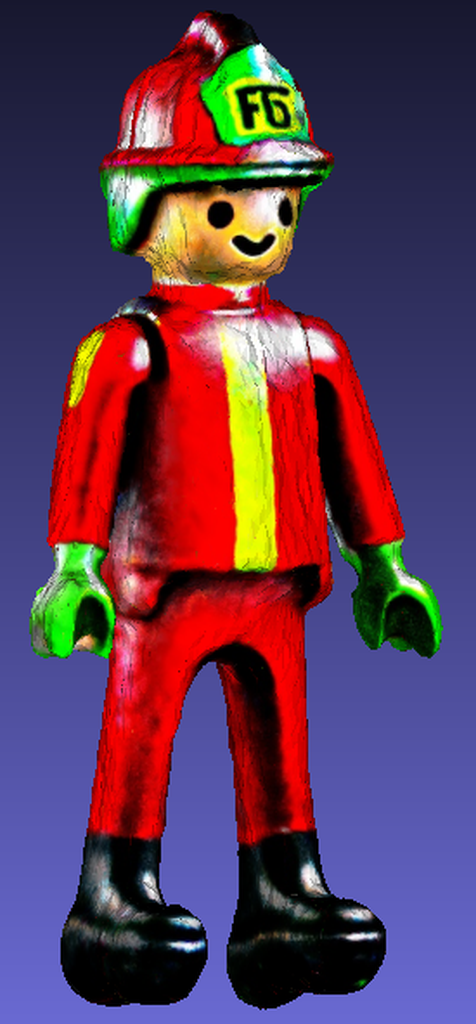
\includegraphics[width=\textwidth]{figures/subjective/magic3d_playmobil_result_resize.png}
        \caption{Magic3D}
    \end{subfigure}
    \begin{subfigure}[b]{0.227\textwidth}
        \centering
        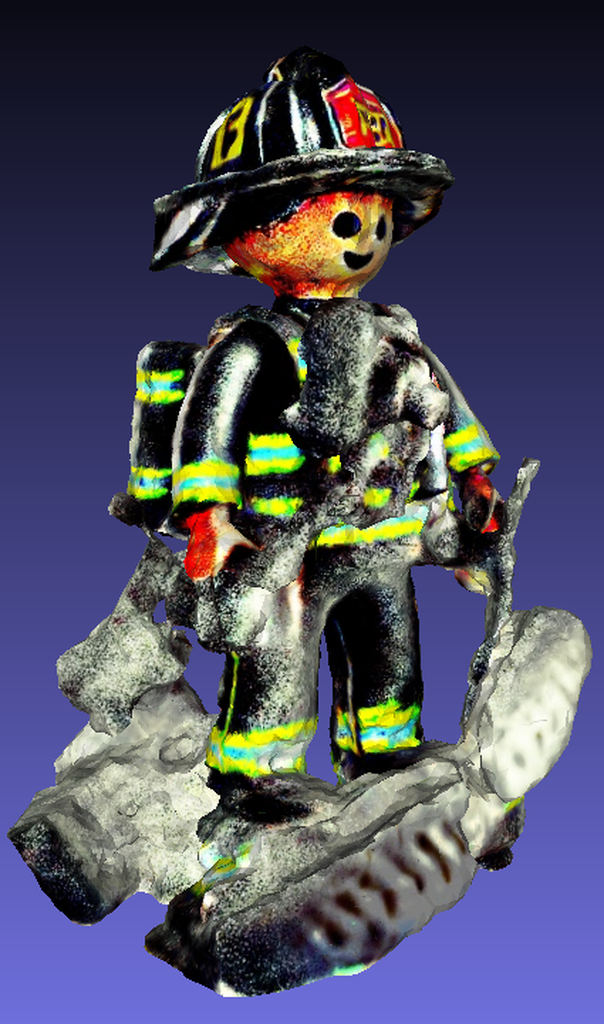
\includegraphics[width=\textwidth]{figures/subjective/fantasia_playmobil_result_resize.png}
        \caption{Fantasta3D}
    \end{subfigure}
    \begin{subfigure}[b]{0.192\textwidth}
        \centering
        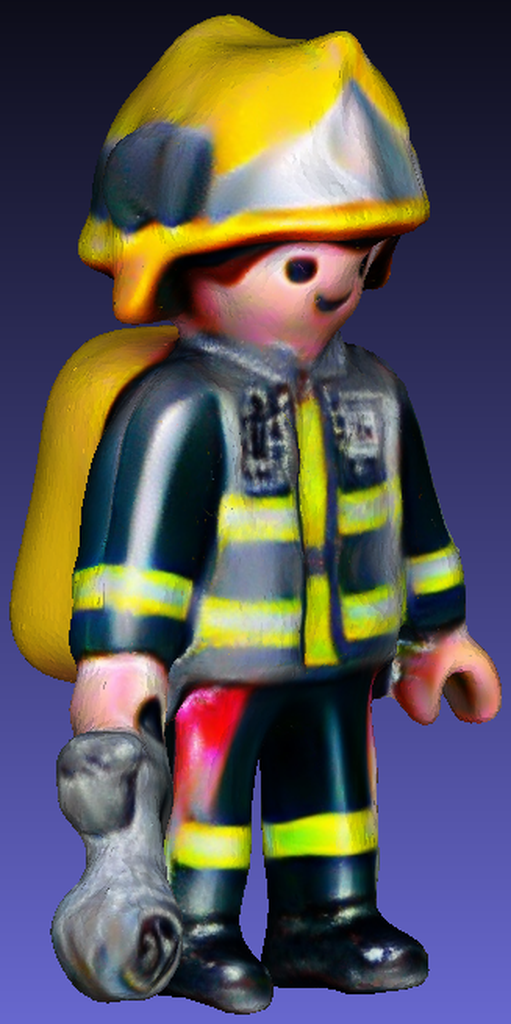
\includegraphics[width=\textwidth]{figures/subjective/magic123_playmobil_result_resize.png}
        \caption{Magic123}
    \end{subfigure}
    \begin{subfigure}[b]{0.181\textwidth}
        \centering
        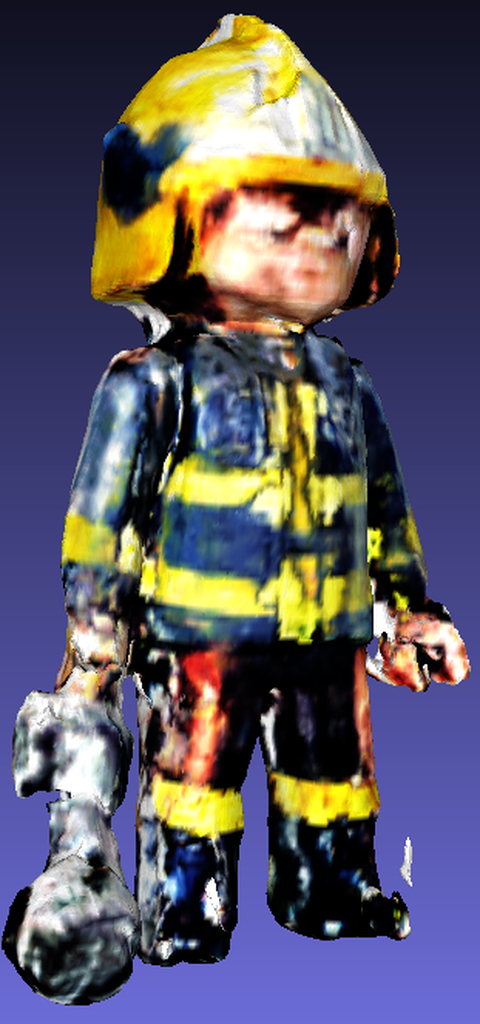
\includegraphics[width=\textwidth]{figures/subjective//wonder3d_playmobil_result_resize.png}
        \caption{Wonder3D}
    \end{subfigure}
    \caption{Results obtained using the prompt ``a high-quality rendering of a Playmobil firefighter''.}~\label{fig:resultPlaymobil}
\end{figure}

\textbf{Prompt/Result Fidelity:} There is a clear split in the results when looking at fidelity to the prompt. DreamFusion and Magic123 tend to stick to the red clothing, while Fantasta3D, Magic123 and Wonder3D opt for a more realistic yellow and black firefighter uniform. Wonder3D and Magic123 adapt their results to the expected color scheme of the input image, given in Figure~\ref{fig:inputPlaymobil} part (a). Of particular interest is Fantasta3D's deviation from the red color scheme, although all models were refined with Stable Diffusion. This can be attributed to the physically based material model in the appearance stage, which has learned to associate firefighter clothing with yellow and black rather than red. Each model successfully reproduces identifiable Playmobil features such as helmets and uniforms, although the extent to which they reproduce the Playmobil style varies.

\textbf{Geometry:} The geometric shape of the models varies significantly. DreamFusion and Wonder3D present the most deviations from the expected Playmobil figure geometry. Both exhibit overly smooth shapes with ambiguous edges and floating elements, such as the hands in DreamFusion and around the right foot in Wonder3D, giving an unfinished appearance. Magic3D impresses with a near-perfect rendering of the Playmobil figure, capturing the sharp transitions at the joints and maintaining smoothness elsewhere, except for a slight distortion around the feet. This result seems like one could bend and move it like it is possible with an original figure. For this prompt, Fantasia3D was initialized with the model derived from Magic3D due to its solid performance, and not with a sphere as is typical. However, this Method still encountered issues with rendering unintended additional objects. These included a presumed fire extinguisher on the back and an ambiguous `thing' at the front, possibly an attempt at rendering a fire hose. Magic123, while delivering a solid representation, introduces a large bag on the figure's back, which, unlike the extraneous parts of Fantasta3D, integrates well with the overall model. A closer look of this bag is given in Figure~\ref{fig:inputPlaymobil} parts (b) and (c). Uniquely, Magic123 recreates the iconic Playmobil hand structure, complete with thumb, fingers, and the characteristic gap between them, capturing the essence of the figure's appendages.

\begin{figure}[ht]
    \centering
    \small
    \begin{subfigure}[b]{0.25\textwidth}
        \centering
        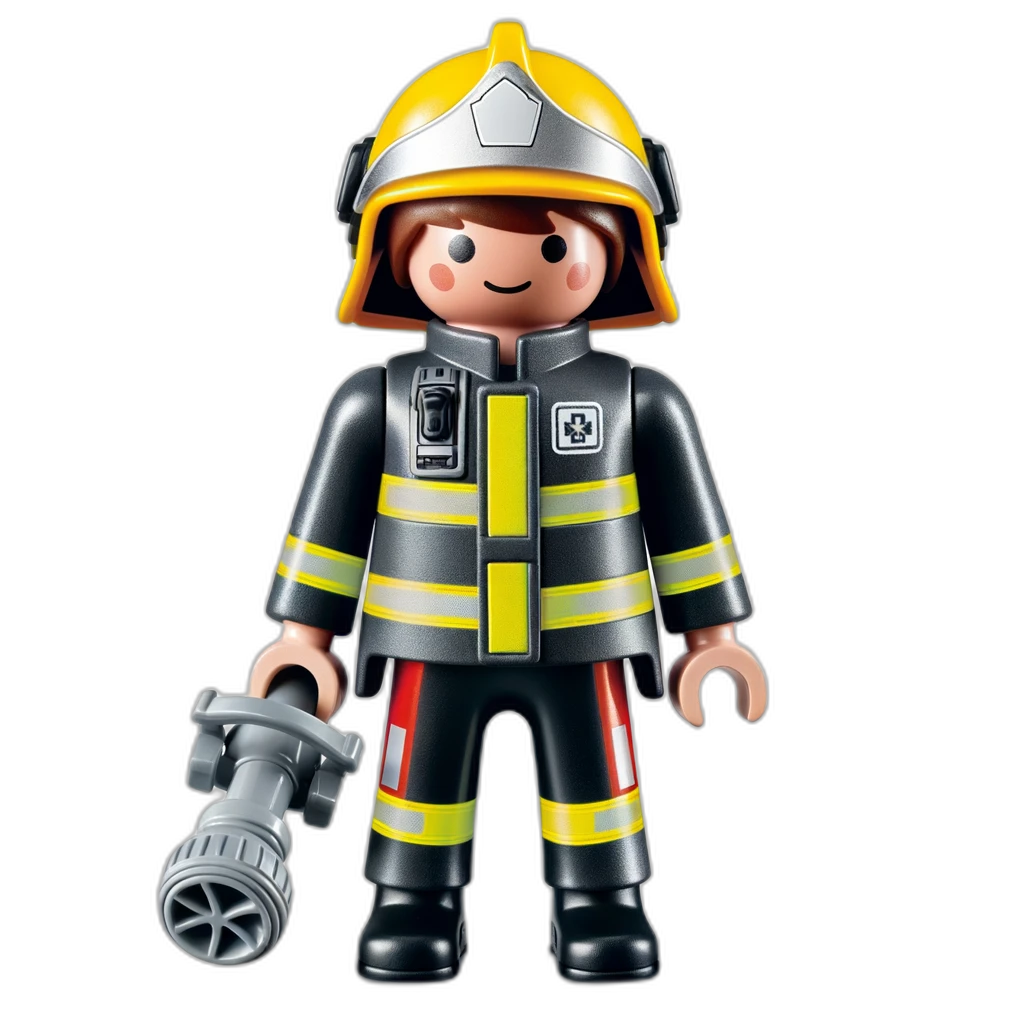
\includegraphics[width=\textwidth]{figures/input/playmobil.png}
        \caption{}
    \end{subfigure}
    \begin{subfigure}[b]{0.25\textwidth}
        \centering
        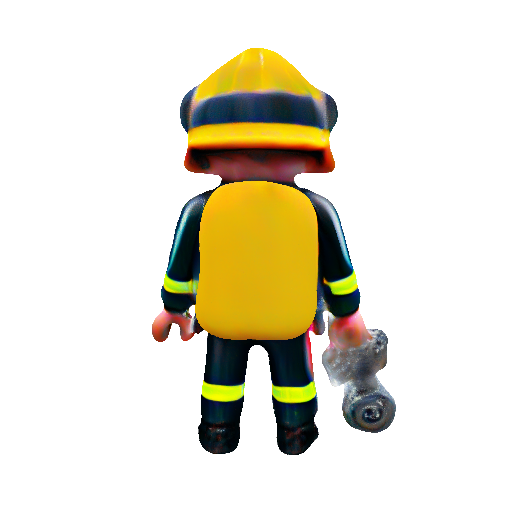
\includegraphics[width=\textwidth]{figures/subjective/magic123_playmobil_refine_back_10000_part1.png}
        \caption{}
    \end{subfigure}
    \begin{subfigure}[b]{0.25\textwidth}
        \centering
        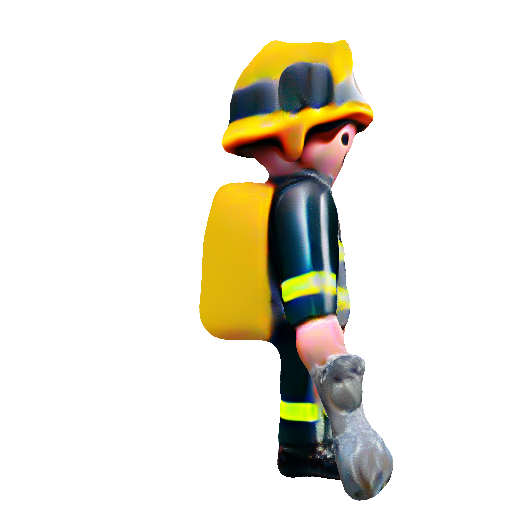
\includegraphics[width=\textwidth]{figures/subjective/magic123_playmobil_refine_right_10000_part1.png}
        \caption{}
    \end{subfigure}
    \caption{Part (a) displays the original image for the Playmobil figure derived form Dall-E 3; Parts (b) and (c) show the side and back view of Magic123, respectively.}~\label{fig:inputPlaymobil}
\end{figure}

\textbf{Texture Realism:} In terms of texture, Magic3D again stands out with a level of realism that surpasses the others for the Playmobil prompt. It is characterized by a clear distinction between the colors, such as the black of the shoes against the red of the uniform, and the face retains the characteristic Playmobil look. The model's interaction with light, evidenced by chest reflections and inner leg shadows, adds to the plastic appearance. DreamFusion's model lacks such light interplay, resulting in a flat appearance, which is also caused due to the overall smoothened geometry. Fantasta3D, Magic123, and Wonder3D diverge from the red texture, opting for a black and yellow combination with realistic reflective stripes. Fantasta3D's texture is sound despite some geometric artifacts, with light reflection indicating a clear light source and giving the helmet a metallic sheen. Magic123 captures a plastic-like sheen, particularly on the arm's reflection, which underscores the roundness and smoothness of the figure. In contrast, Wonder3D's texture is not very detailed, blurs differences like the separation between jacket and shirt and does not render the character's face, similar to DreamFusion. The whole model looks strange, decayed and unfinished.

The results of this prompt show that DreamFusion struggles with detailed geometry, resulting in smooth and inaccurate shapes, but still offers acceptable color fidelity. Magic3D, on the other hand, excels in both realistic textures and geometric accuracy, especially when the prompt specifies a flat structure and no intricate detail is required. Fantasta3D tends to render overly realistic models, often at the expense of key prompt features, resulting in unnecessary additions in both geometry and appearance. Similarly, Magic123, while generally rendering the essence of the prompt well, tends to add unnecessary elements such as the unexpected bag. Finally, Wonder3D fails to produce even basic details, resulting in models that look unfinished and incomplete.\\




The next prompt used for the various methods was \textbf{``a rendering of a highly symmetrical loaf of bread''}. This prompt was selected to test the precision of each method in replicating detailed, specific requests while still producing coherent results. In this case, the model was tested for its symmetric result capability, which is discussed later in the technical section. The generated models are displayed in Figure~\ref{fig:resultBread}, which also includes the original input image created by Dall-E 3 in part (f).

\begin{figure}[ht]
    \centering
    \small
    \begin{subfigure}[b]{0.31\textwidth}
        \centering
        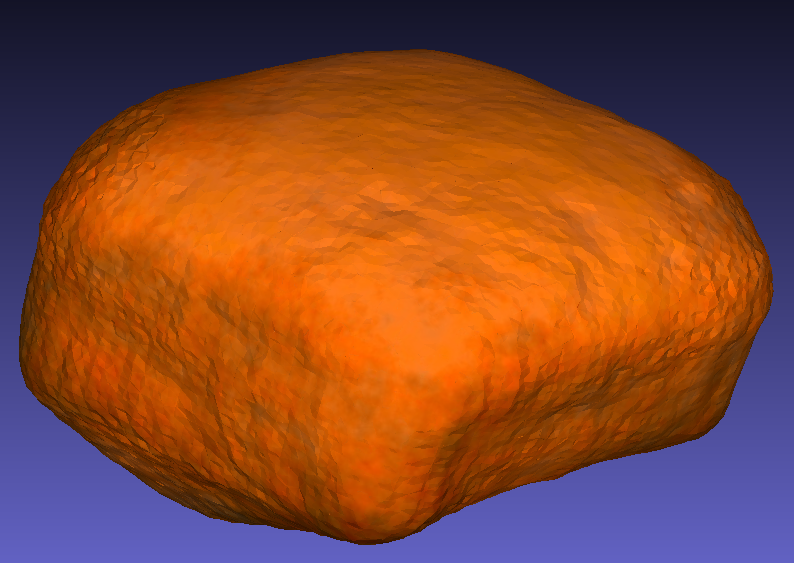
\includegraphics[width=\textwidth]{figures/subjective/dreamfusion_bread_result.png}
        \caption{DreamFusion}
        \vspace{0.1cm}
    \end{subfigure}
    \begin{subfigure}[b]{0.31\textwidth}
        \centering
        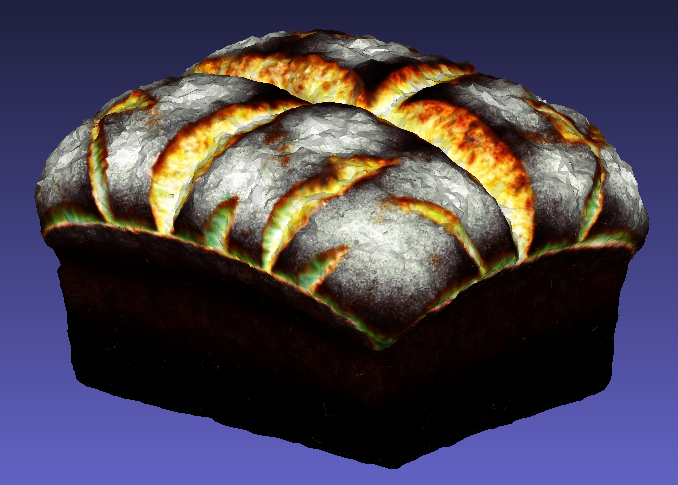
\includegraphics[width=\textwidth]{figures/subjective/magic3D_bread_result.png}
        \caption{Magic3D}
        \vspace{0.1cm}
    \end{subfigure}
    \begin{subfigure}[b]{0.2\textwidth}
        \centering
        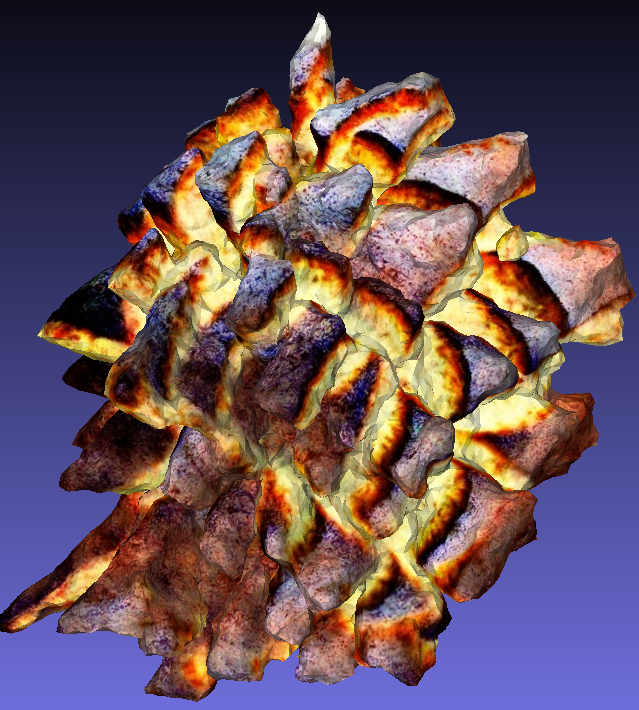
\includegraphics[width=\textwidth]{figures/subjective/fantasia_bread_result.png}
        \caption{Fantasta3D}
        \vspace{0.1cm}
    \end{subfigure}

    \begin{subfigure}[b]{0.269\textwidth}
        \centering
        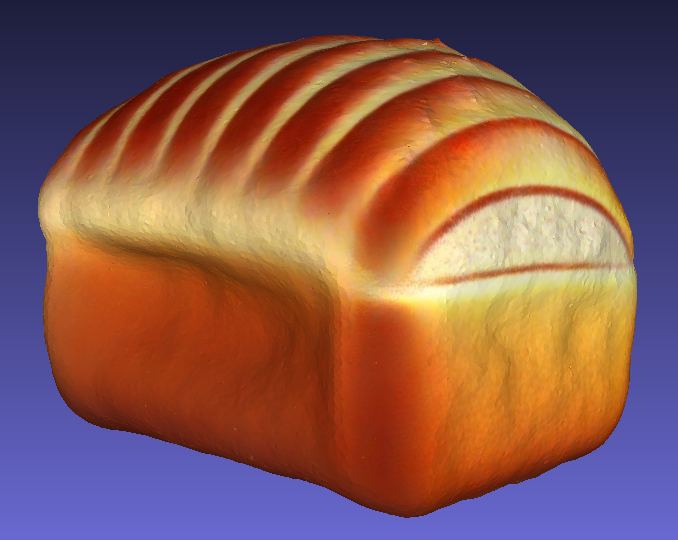
\includegraphics[width=\textwidth]{figures/subjective/magic123_bread_result.png}
        \caption{Magic123}
        \vspace{0.1cm}
    \end{subfigure}
    \begin{subfigure}[b]{0.23\textwidth}
        \centering
        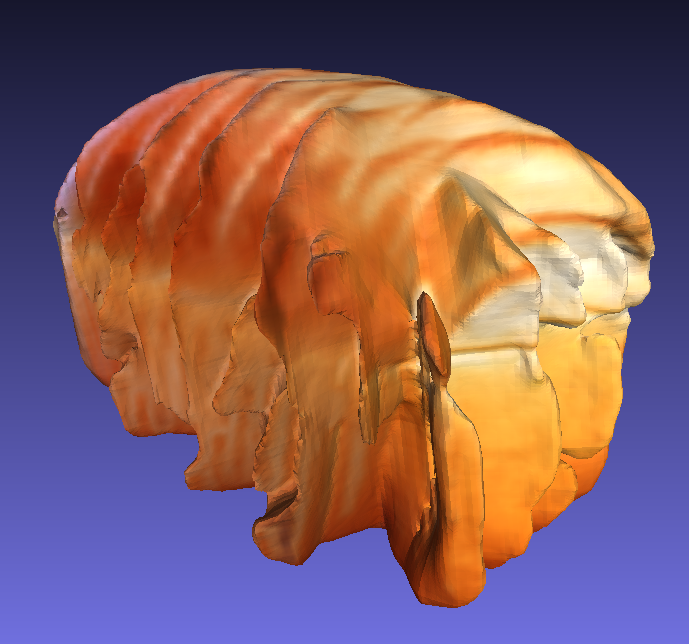
\includegraphics[width=\textwidth]{figures/subjective/wonder3d_bread_result.png}
        \caption{Wonder3D}
        \vspace{0.1cm}
    \end{subfigure}
    \begin{subfigure}[b]{0.23\textwidth}
        \centering
        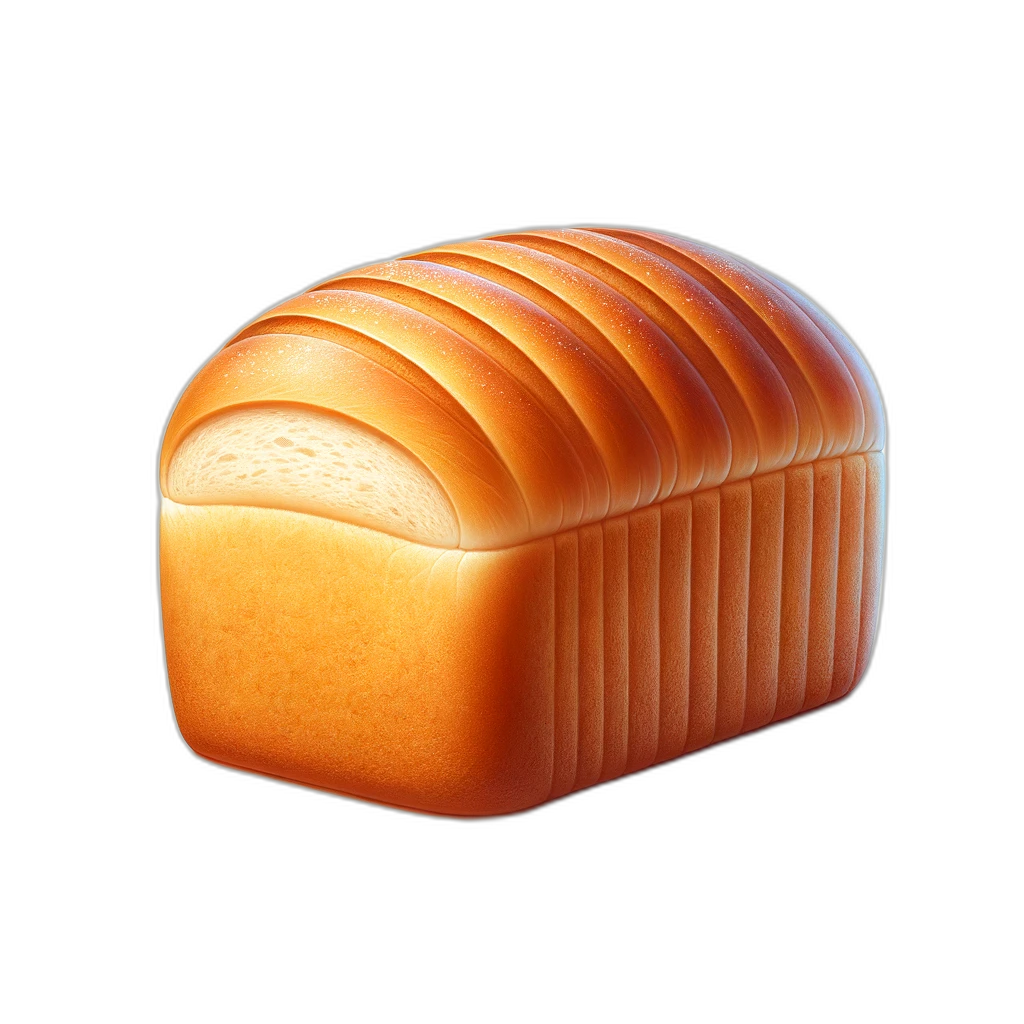
\includegraphics[width=\textwidth]{figures/input/bread.png}
        \caption{Original Image}
        \vspace{0.1cm}
    \end{subfigure}
    \caption{Results obtained using the prompt ``a rendering of a highly symmetrical loaf of bread''. Part (f) is the input image for Magic123 and Wonder3D, generated with Dall-E 3}~\label{fig:resultBread}
\end{figure}

Regarding \textbf{Prompt/Result Fidelity}, the outcomes varied. Magic123 and Magic3D successfully captured the essence of a bread, while Wonder3D produced a result that only vaguely suggested a loaf of bread. DreamFusion and Fantasia3D, however, were less successful; the former's result was indistinct, resembling a nondescript lump, while the latter's output more closely resembled a pineapple or an explosion when viewed without context.

In terms of \textbf{Geometry}, DreamFusion's model lacked meaningful structure, while Magic3D's bread model achieved good geometry, with a realistically carved top resembling fresh black bread. Fantasia3D, on the other hand, produced a model with a spikey appearance, potentially due to overfitting or difficulty in determining a starting point for the flat bottom of the bread. Magic123 excelled in replicating the geometry of the input image, closely matching the cuts and overall shape of the bread. Conversely, Wonder3D's model, like Fantasia3D's, had a roughly bread-like shape but suffered from spikey edges, possibly due to small adjustments during 3D mesh generation.

When considering \textbf{Texture Realism}, only the textures from Magic3D, Fantasia3D, and Magic123 seemed noteworthy. Magic3D's texture gave the impression of a burnt, dark loaf, with a realistic color gradient on the top. Although Fantasia3D's texture had a pleasing color combination, it resembled a cluster of breadsticks unless contextual information was provided. Magic123 accurately replicated the texture of the original image, demonstrating its proficiency in handling low-detail requirements.

To summarize, DreamFusion continues to have issues with structure, suggesting that direct prompts for certain features such as symmetry may lead to confusion rather than better results. Magic3D maintained its solid performance, suggesting that some level of directives in the prompt can be beneficial. Fantasia3D appeared to be thrown off by the specific prompt, resulting in poorer results compared to previous tasks. Magic123's exact replication of the input image leaves the impact of the specific prompt on its performance unclear. Wonder3D again struggled to accurately generate the overall structure, reflecting ongoing challenges in model training.\\





To evaluate the capability of various methods in rendering organic forms and textures, the prompt \textbf{``a high-quality rendering of a big dog sleeping on a chair''} was used. This prompt was specifically chosen to test the realism of fur texture and the anatomical accuracy of a resting dog. This setup also provided an opportunity to observe the effectiveness of multiview-consistency, a feature in Wonder3D, in enhancing the quality of the outputs.

For \textbf{Prompt/Result Fidelity}, most models, except DreamFusion, produced a recognizable dog, as evidenced in Figure~\ref{fig:resultDogFront} and~\ref{fig:resultDogBack}. However, all text-to-3D methods struggled with accurately rendering the chair's backrest, with Fantasia3D notably failing to make it clear what the dog was even resting on. Image-to-3D methods, Magic123 and Wonder3D, provided solid front views of the scene, though Magic123's representation from behind showed an unusually inflated and rounded chair shape.

\begin{figure}[ht]
    \centering
    \small
    \begin{subfigure}[b]{0.295\textwidth}
        \centering
        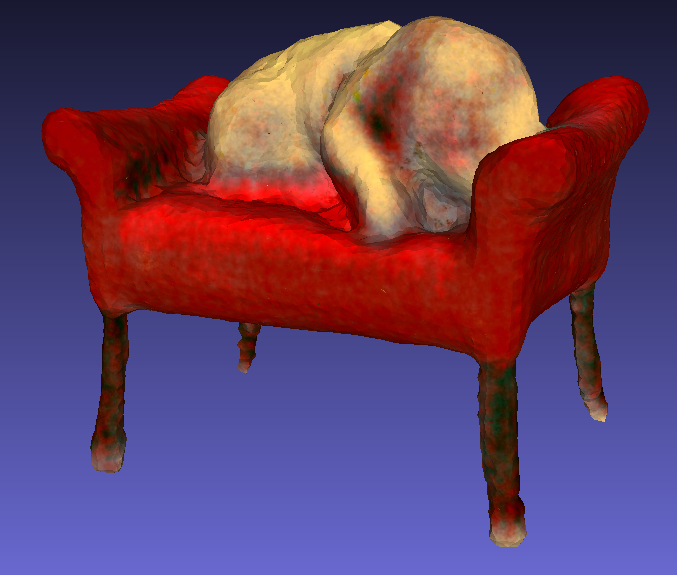
\includegraphics[width=\textwidth]{figures/subjective/dreamfusion_dog_front_result.png}
        \caption{DreamFusion}
        \vspace{0.1cm}
    \end{subfigure}
    \begin{subfigure}[b]{0.32\textwidth}
        \centering
        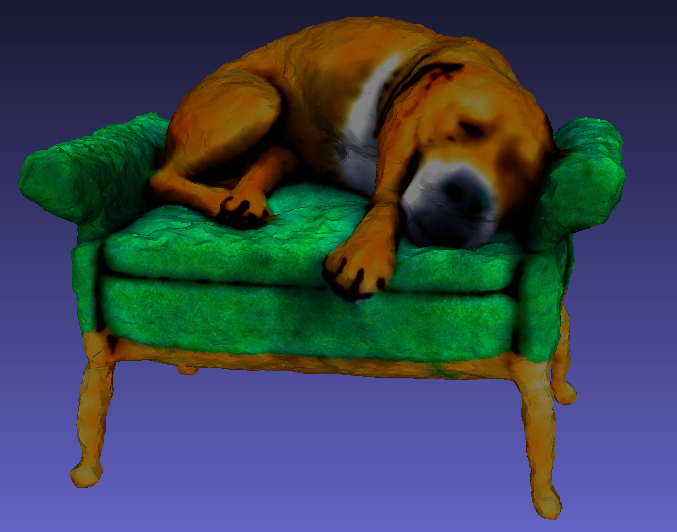
\includegraphics[width=\textwidth]{figures/subjective/magic3D_dog_front_result.png}
        \caption{Magic3D}
        \vspace{0.1cm}
    \end{subfigure}
    \begin{subfigure}[b]{0.33\textwidth}
        \centering
        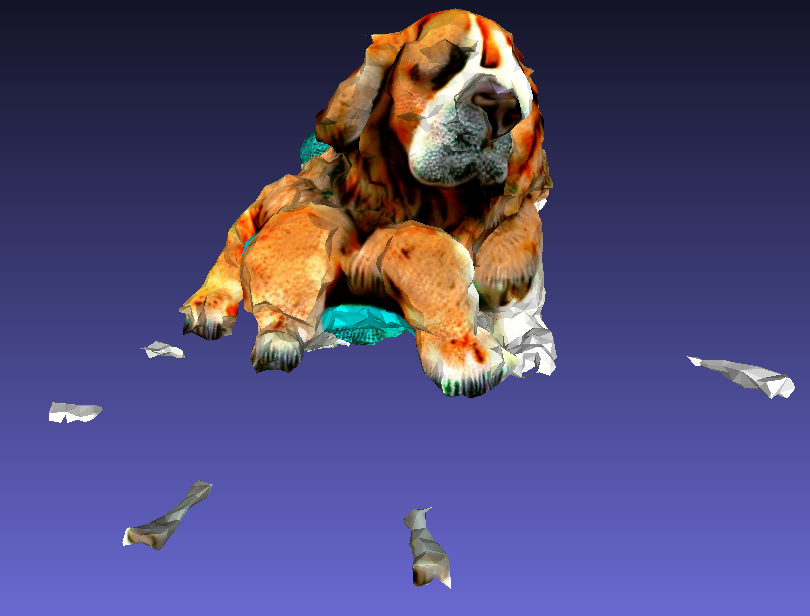
\includegraphics[width=\textwidth]{figures/subjective/fantasia_dog_front_result.png}
        \caption{Fantasta3D}
        \vspace{0.1cm}
    \end{subfigure}

    \begin{subfigure}[b]{0.267\textwidth}
        \centering
        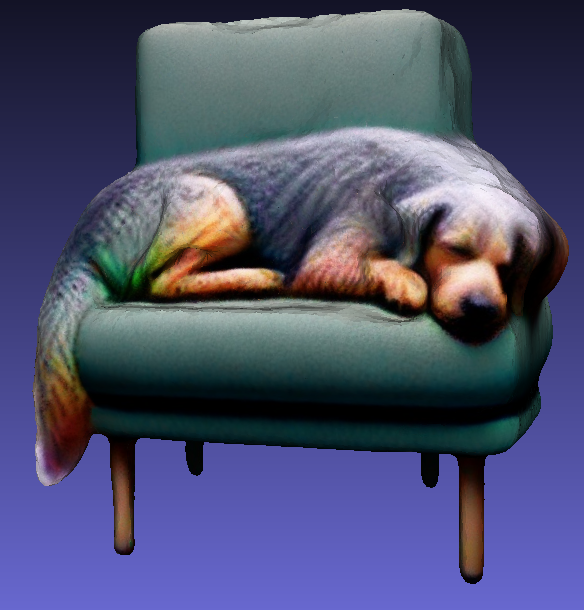
\includegraphics[width=\textwidth]{figures/subjective/magic123_dog_front_result.png}
        \caption{Magic123}
        \vspace{0.1cm}
    \end{subfigure}
    \begin{subfigure}[b]{0.27\textwidth}
        \centering
        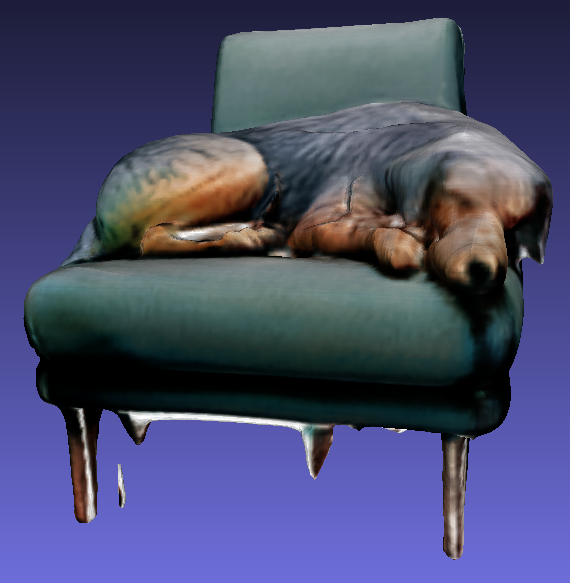
\includegraphics[width=\textwidth]{figures/subjective/wonder3D_dog_front_result.png}
        \caption{Wonder3D}
        \vspace{0.1cm}
    \end{subfigure}
    \begin{subfigure}[b]{0.28\textwidth}
        \centering
        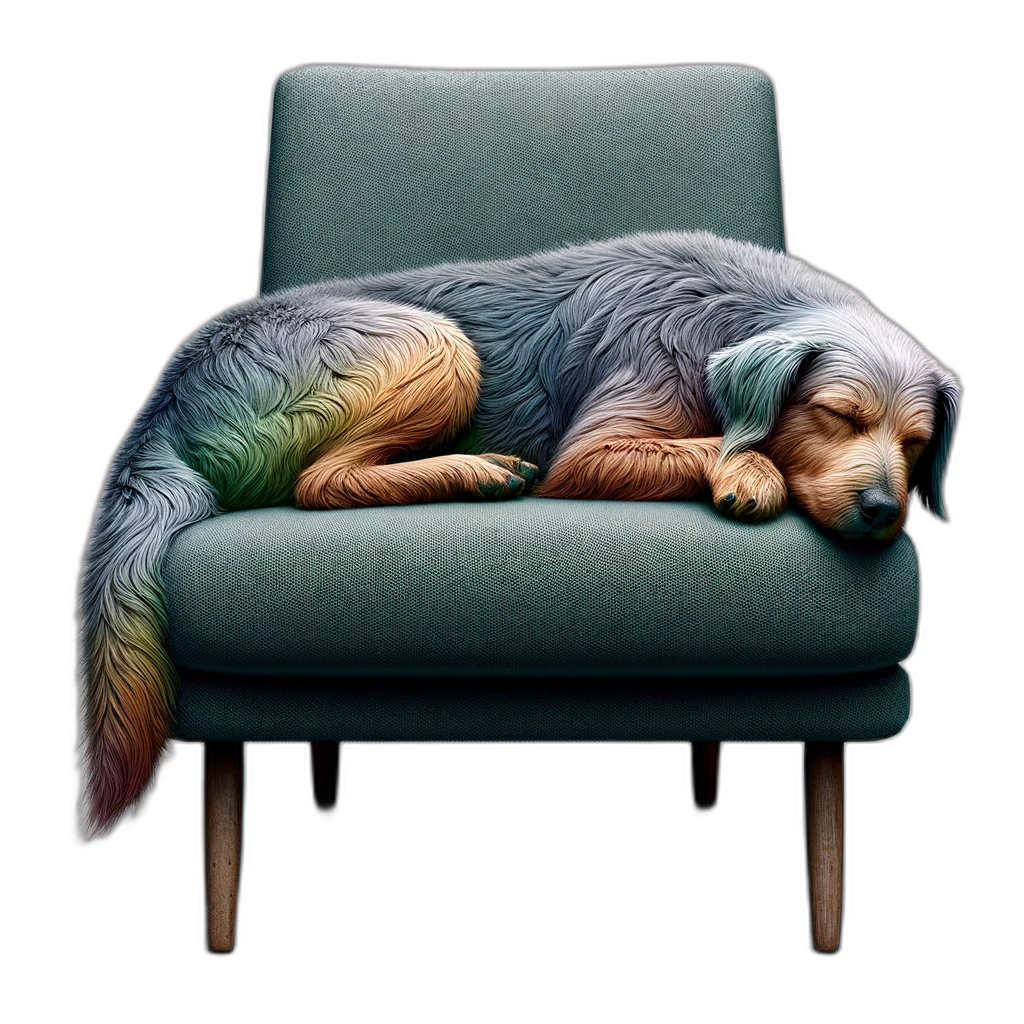
\includegraphics[width=\textwidth]{figures/input/dog.png}
        \caption{Original Image}
        \vspace{0.1cm}
    \end{subfigure}
    \caption{The front view of the generated objects with the prompt ``a high-quality rendering of a big dog sleeping on a chair''.}~\label{fig:resultDogFront}
\end{figure}

In the aspect of \textbf{Geometry}, DreamFusion had difficulties rendering a recognizable dog shape, unlike the other methods. Magic3D's output was more successful, clearly differentiating between the dog and the chair from both front and back views, although an anomaly was noted where the dog appeared to have a total of four back legs in different views. This issue could stem from Magic3D's lack of multi-view consistency, in contrast to Wonder3D. Fantasia3D's model showed a dog, but with less detail and shape accuracy, especially in the front view where the legs seemed to emerge directly from the neck. Both Magic123 and Wonder3D did an impressive job of capturing the main features of the input image in the front view, as can be seen in part (f) of Figure~\ref{fig:resultDogFront}. However, viewing from the back side, Magic123's rendering of the chair was less convincing, whereas Wonder3D's multi-view consistency resulted in a more accurate and flat back of the chair, despite some missing chair legs and floating parts.\\

For \textbf{Texture Realism}, each method displayed distinct capabilities and limitations. DreamFusion's texture lacked explicit detail, resulting in a smoothed-out appearance that made it difficult to discern a dog lying on a chair. This lack of detail in texture diminished the overall realism of the scene. Magic3D, while not offering much depth in texture of the fur, managed to convey the impression of a dog through its effective use of color variations. The distinctions between the brown fur, black nose, paw gaps, shadows, and the white of the dog's neck and belly were clear, creating a convincing representation of a dog despite the geometric inaccuracies. Fantasia3D, although its geometric output was less accurate, excelled in texture detail. The color variations across the dog's face were more nuanced compared to Magic3D, adding a layer of realism. Even with the structural issues, the texture applied depth to the model and gave it a lifelike appearance of a dog. Magic123 and Wonder3D both achieved similar levels of detail in texture, closely mirroring the input image. Magic123, however, introduced additional lighting into the scene. This was evident in the reflections on the dog's back and face, enhancing the vitality of the overall scene. The texture of the chair's backrest was much finer Wonder3D and benefited from the interplay between shadow and light. This attention to detail made the fabric of the chair appear better.

\begin{figure}[ht]
    \centering
    \small
    \begin{subfigure}[b]{0.291\textwidth}
        \centering
        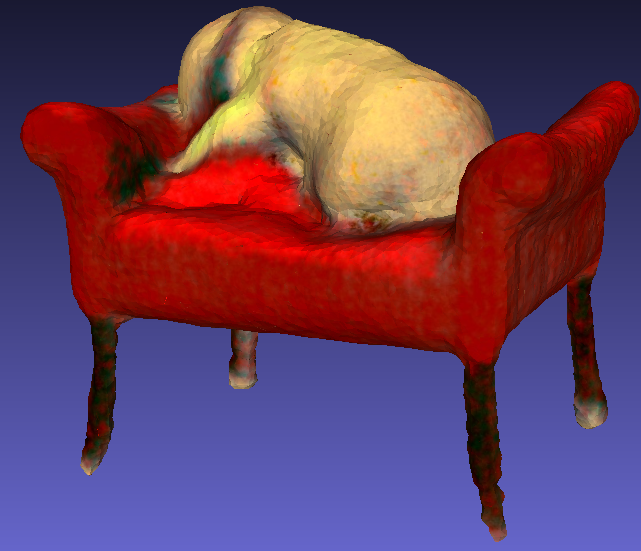
\includegraphics[width=\textwidth]{figures/subjective/dreamfusion_dog_back_result.png}
        \caption{DreamFusion}
        \vspace{0.1cm}
    \end{subfigure}
    \begin{subfigure}[b]{0.3\textwidth}
        \centering
        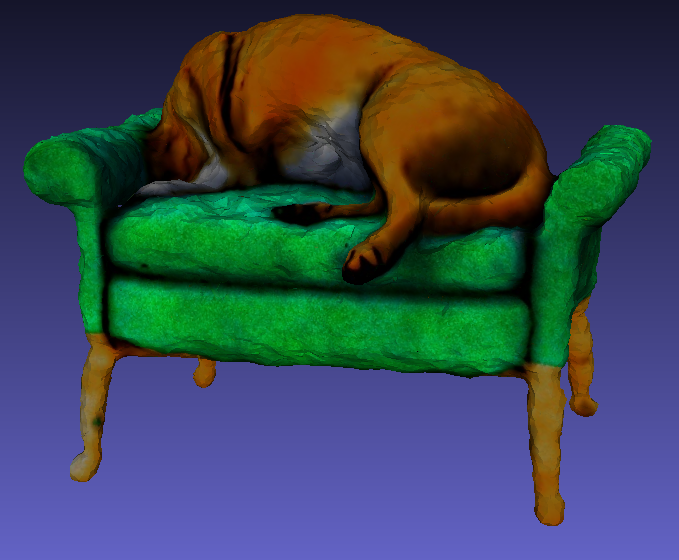
\includegraphics[width=\textwidth]{figures/subjective/magic3D_dog_back_result.png}
        \caption{Magic3D}
        \vspace{0.1cm}
    \end{subfigure}
    \begin{subfigure}[b]{0.34\textwidth}
        \centering
        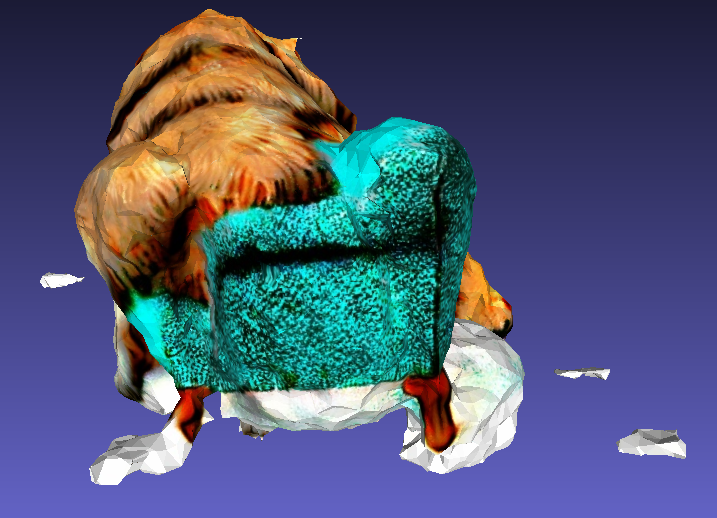
\includegraphics[width=\textwidth]{figures/subjective/fantasia_dog_back_result.png}
        \caption{Fantasta3D}
        \vspace{0.1cm}
    \end{subfigure}

    \begin{subfigure}[b]{0.261\textwidth}
        \centering
        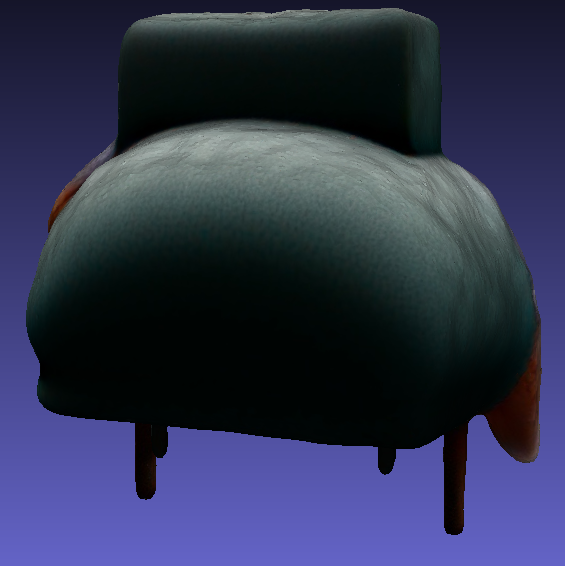
\includegraphics[width=\textwidth]{figures/subjective/magic123_dog_back_result.png}
        \caption{Magic123}
        \vspace{0.1cm}
    \end{subfigure}
    \begin{subfigure}[b]{0.27\textwidth}
        \centering
        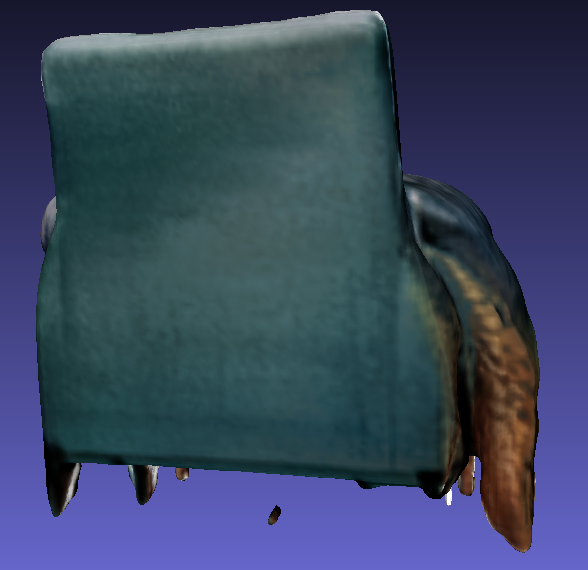
\includegraphics[width=\textwidth]{figures/subjective/wonder3D_dog_back_result.png}
        \caption{Wonder3D}
        \vspace{0.1cm}
    \end{subfigure}
    \caption{The back view of the prompt ``a high-quality rendering of a big dog sleeping on a chair''}~\label{fig:resultDogBack}
\end{figure}

DreamFusion again presented the lowest level of detail, failing to recognize the object specified in the prompt. Magic3D effectively captured the required elements, including the dog's resting anatomy, yet produced a flat, depthless texture for the fur. Fantasia3D accurately rendered parts of the prompt, focusing on the dog, striving for realistic texture but faltering in basic geometric accuracy. Magic123 performed well in replicating the shape from the original image but struggled with rendering views different from the input. Wonder3D solidly recreated the input image, offering a consistent shape and texture from multiple viewpoints.\\






To delve deeper into each method's ability to render complex elements and contrasting materials, the prompt \textbf{``a high-quality rendering of a fern in a wooden pot''} was introduced. While plants had been used previously to illustrate each method's generation process, there hadn't been a comparison between the various Methods. This prompt aimed to evaluate how each method handled intricate details in natural subjects and the accuracy of color gradients and lighting in varying depths. The outcomes of this exercise are displayed in Figure~\ref{fig:resultFern}.

\begin{figure}[ht]
    \centering
    \small
    \begin{subfigure}[b]{0.24\textwidth}
        \centering
        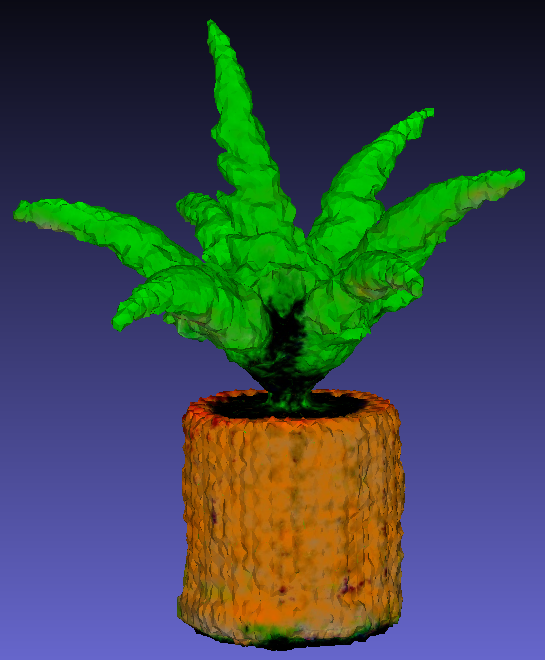
\includegraphics[width=\textwidth]{figures/subjective/dreamfusion_fern_result.png}
        \caption{DreamFusion}
        \vspace{0.1cm}
    \end{subfigure}
    \begin{subfigure}[b]{0.35\textwidth}
        \centering
        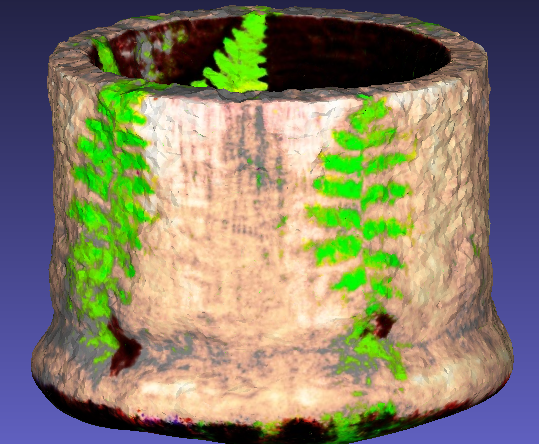
\includegraphics[width=\textwidth]{figures/subjective/magic3d_fern_result.png}
        \caption{Magic3D}
        \vspace{0.1cm}
    \end{subfigure}
    \begin{subfigure}[b]{0.32\textwidth}
        \centering
        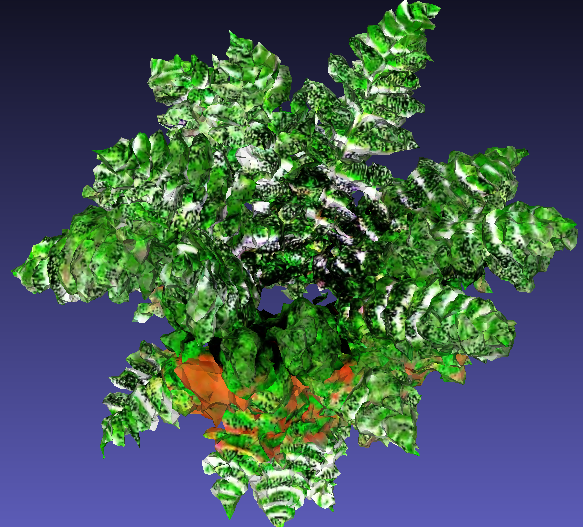
\includegraphics[width=\textwidth]{figures/subjective/fantasia_fern_result.png}
        \caption{Fantasta3D}
        \vspace{0.1cm}
    \end{subfigure}

    \begin{subfigure}[b]{0.28\textwidth}
        \centering
        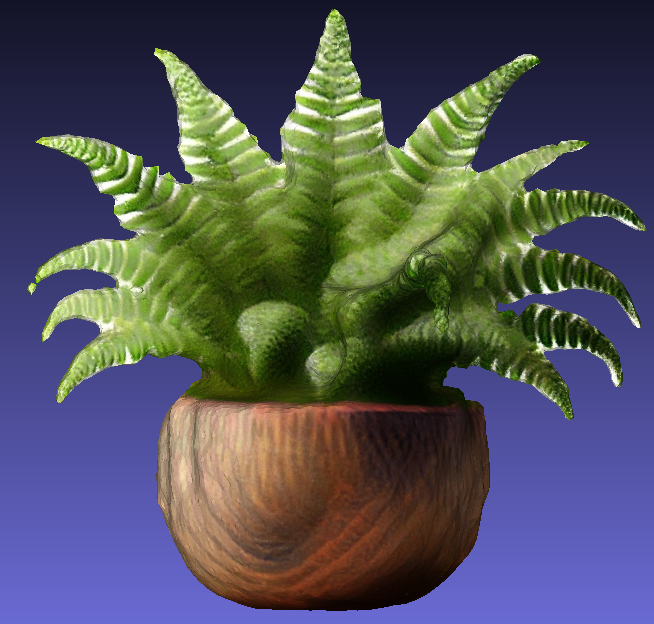
\includegraphics[width=\textwidth]{figures/subjective/magic123_fern_front_result.png}
        \caption{Magic123}
        \vspace{0.1cm}
    \end{subfigure}
    \begin{subfigure}[b]{0.27\textwidth}
        \centering
        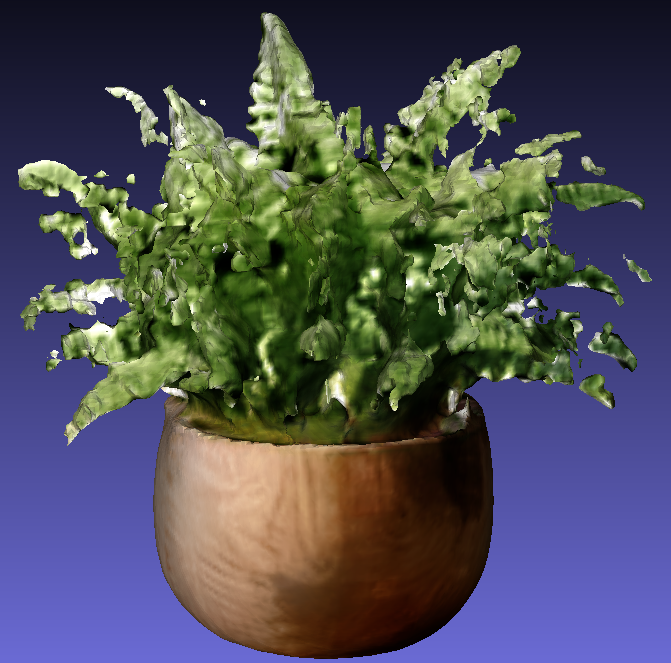
\includegraphics[width=\textwidth]{figures/subjective/wonder3d_fern_result.png}
        \caption{Wonder3D}
        \vspace{0.1cm}
    \end{subfigure}
    \begin{subfigure}[b]{0.28\textwidth}
        \centering
        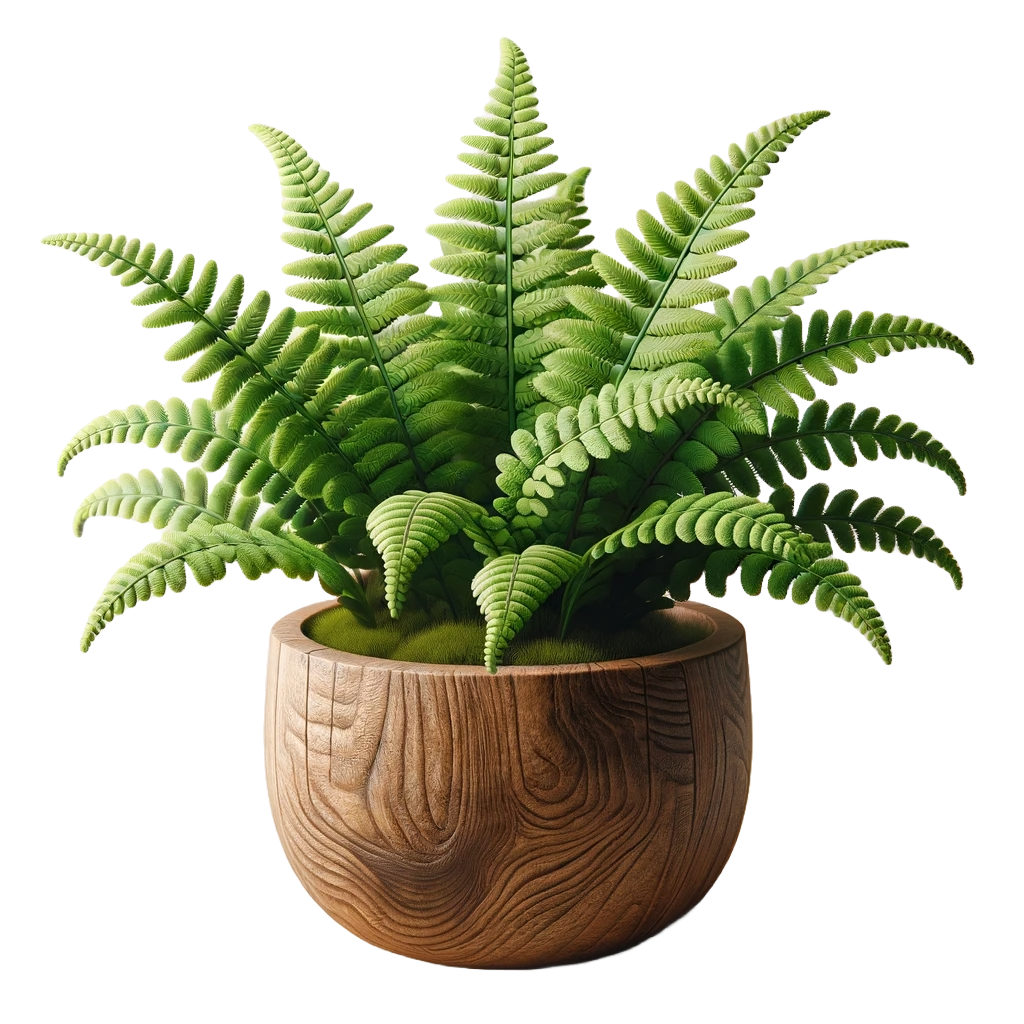
\includegraphics[width=\textwidth]{figures/input/fern.png}
        \caption{Original Image}
        \vspace{0.1cm}
    \end{subfigure}
    \caption{Results obtained using the prompt ``a high-quality rendering of a fern in a wooden pot''.}~\label{fig:resultFern}
\end{figure}

In terms of \textbf{Prompt/Result Fidelity}, DreamFusion presented a fern and wooden pot that were recognizable, though it was debatable whether the plant could be distinctly identified as a fern. Magic3D struggled, failing to generate the fern and only displaying the pot with a texture vaguely resembling a fern. Interestingly, earlier in the coarse training, the fern was part of the model and was rendered, as seen in Figure~\ref{fig:fernSideview}, part (a). Fantasia3D showed a detailed fern but didn't render the wooden pot well. Magic123's front view effectively depicted both the fern and pot, but the side view lacked volume, making the plant appear flat compared to Wonder3D, which displayed a solid result for both the plant and pot from all angles, thanks to its multi-view consistency. The side views of Magic123 and Wonder3D are depicted in part (b) and (c) in Figure~\ref{fig:fernSideview}.\\

Regarding \textbf{Geometry}, DreamFusion's model convincingly resembled a plant from all angles, with clear distinction between the pot and plant. Magic3D's pot was well-rendered with true shape and structure, but the plant went completely missing after the refinement stage. Fantasia3D exhibited detailed fern parts but failed to accurately portray the pot. Magic3D's model had a good pot shape, but the plant appeared flat and overly smoothed, possibly due to limitations in the input image, as white parts remained at the edges after the background was removed. Wonder3D presented a well-formed fern and pot from all views, although some floating parts and mixed-up sections were noticeable at a closer look.

For \textbf{Texture Realism}, DreamFusion's model allowed for basic identification of the pot as brown and the plant as green but lacked in shading and detail. Magic3D displayed three detailed fern leaves on the pot, but with incorrect positioning and lack of color variation due to the shape flaws. Fantasia3D achieved a realistic plant texture with significant depth and color variation, although the pot's color was less distinct. Magic123's texture appeared smooth with low detail in the plants, though the shadows and pot color matched well with the original image. Wonder3D showed detailed and varied colors within the plant, indicating depth, but the overall texture quality diminished upon closer inspection. However, the color consistency across all viewpoints and the well-rendered pot compared to the original image were notable strengths.

\begin{figure}[ht]
    \centering
    \small
    \begin{subfigure}[b]{0.35\textwidth}
        \centering
        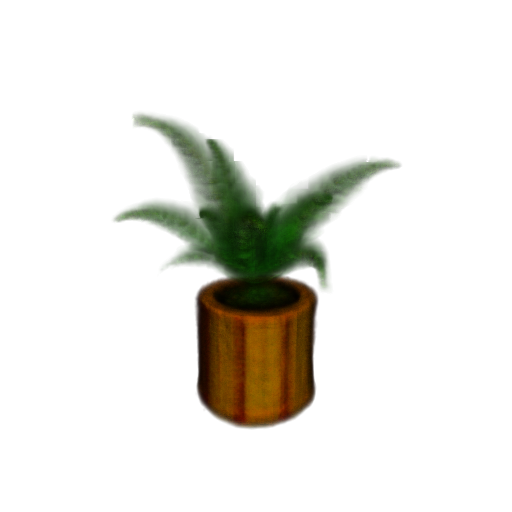
\includegraphics[width=\textwidth]{figures/subjective/magic3D_fern_coarse_part1.png}
        \caption{Magic3D~-~coarse}
    \end{subfigure}
    \begin{subfigure}[b]{0.2\textwidth}
        \centering
        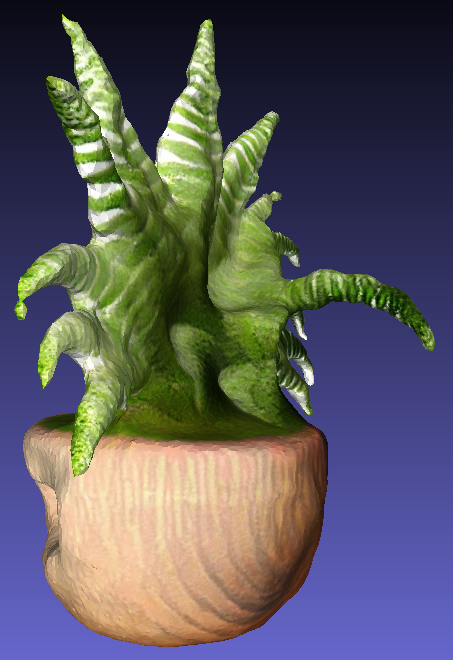
\includegraphics[width=\textwidth]{figures/subjective/magic123_fern_side_result.png}
        \caption{Magic123}
    \end{subfigure}
    \begin{subfigure}[b]{0.32\textwidth}
        \centering
        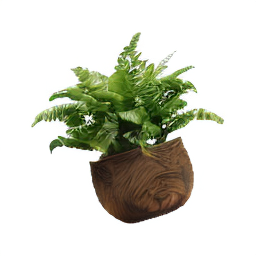
\includegraphics[width=\textwidth]{figures/subjective/rgb_000_right.png}
        \caption{Wonder3D}
    \end{subfigure}
    \caption{Part (a) shows the result of the coarse stage of Magic3D, where the actual fern was still present; (b and c) show the side view of the fern showcasing the limitations of Magic123 in deriving the correct angles in contrast to Wonder3D}\label{fig:fernSideview}
  \end{figure}

In summary, DreamFusion captured the basic shape and texture but lacked fine details, depth, and color variation, suggesting difficulty with intricate requests. Magic3D failed to accurately render detailed objects from the prompt, leading to an unsatisfactory output. Fantasia3D again achieved the most realistic texture but fell short in basic geometric aspects. Magic123 covered the basics, mirroring the view from the input image, but lacked detail, resulting in a flat, undetailed appearance. Wonder3D succeeded in capturing the basic form from all angles, with reasonable depth and structure. However, upon closer inspection, the texture appeared undetailed, and floating parts were noticeable.\\



The final prompt given to the methods was \textbf{``a detailed rendering of a snow globe containing a snowman''}, aimed at testing each method's ability to handle transparency and difficult reflections of glass. This prompt also evaluated the capacity to generate objects within other objects, like a snowman inside a glass globe. The results are depicted in Figure~\ref{fig:resultGlobe}.

In terms of \textbf{Prompt/Result Fidelity}, no method could successfully render transparent glass with objects inside. This limitation might stem from the NeRFs' sampling process, where each view translates into a 2D image, potentially leading to a loss of three-dimensional structure information. Surprisingly, DreamFusion came closest to achieving the goal, capturing the intended object but failing to render the glass dome of the snow globe

Analyzing \textbf{Geometry}, there were significant difficulties across most methods.  DreamFusion presented a well-structured podium and snowman, albeit lacking in detail and missing the glass dome. During training, this method depicted the dome with multiple floating parts representing one globe, as seen in Figure~\ref{fig:dreamfusionGlobe}. However, these parts were removed in mesh conversion. Magic3D failed to produce a valid globe, resulting in an oval rather than a round shape. Fantasia3D seemed to focus more on the snowman, with an oversized belly potentially mistaken for the globe, and an inaccurately shaped snowman with legs and feet. Magic123's front view was promising, closely resembling the input image, but the side view, as seen in Figure 32, part (c), showed a thinner globe. Wonder3D stood out in its geometry rendering, presenting a circular dome from all viewpoints. Minor inconsistencies were observed at the bowl's connection to the podium, but these were minor compared to the other methods.

\begin{figure}[ht]
    \centering
    \small
    \begin{subfigure}[b]{0.232\textwidth}
        \centering
        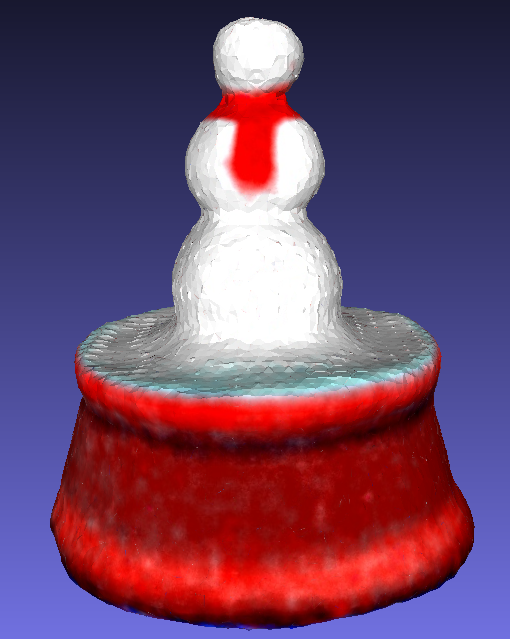
\includegraphics[width=\textwidth]{figures/subjective/dreamfusion_globe_result.png}
        \caption{DreamFusion}
        \vspace{0.1cm}
    \end{subfigure}
    \begin{subfigure}[b]{0.17\textwidth}
        \centering
        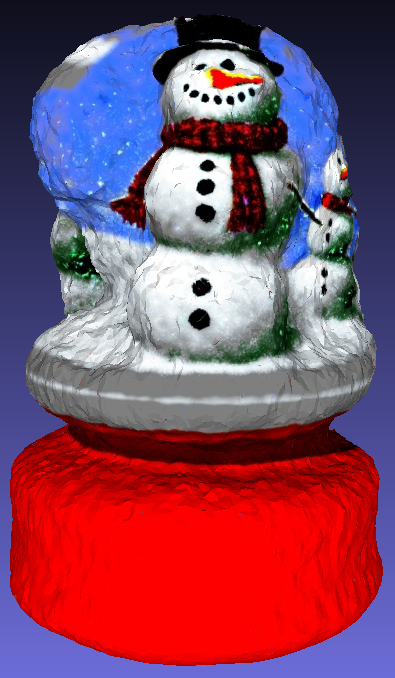
\includegraphics[width=\textwidth]{figures/subjective/magic3d_globe_result.png}
        \caption{Magic3D}
        \vspace{0.1cm}
    \end{subfigure}
    \begin{subfigure}[b]{0.241\textwidth}
        \centering
        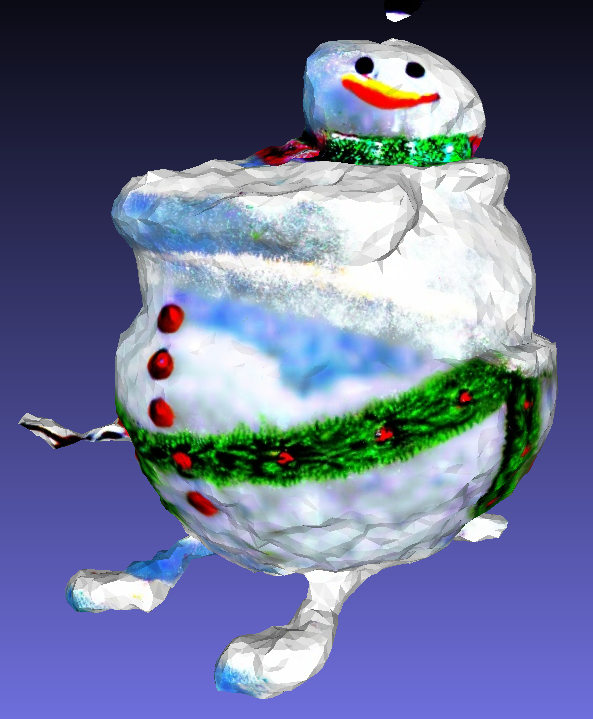
\includegraphics[width=\textwidth]{figures/subjective/fantasia3d_globe_result.png}
        \caption{Fantasta3D}
        \vspace{0.1cm}
    \end{subfigure}

    \begin{subfigure}[b]{0.234\textwidth}
        \centering
        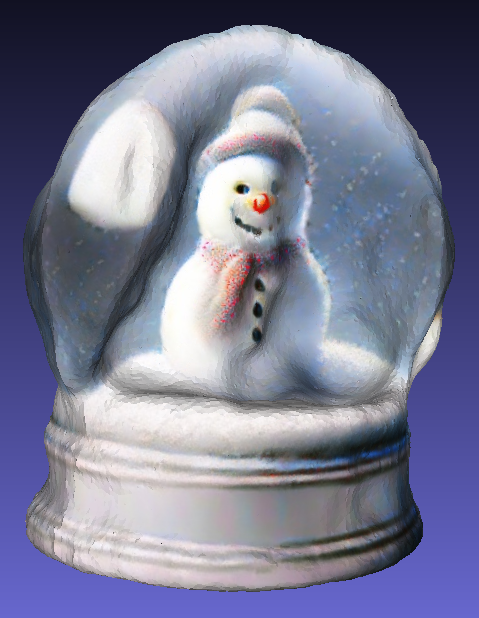
\includegraphics[width=\textwidth]{figures/subjective/magic123_globe_result.png}
        \caption{Magic123}
        \vspace{0.1cm}
    \end{subfigure}
    \begin{subfigure}[b]{0.27\textwidth}
        \centering
        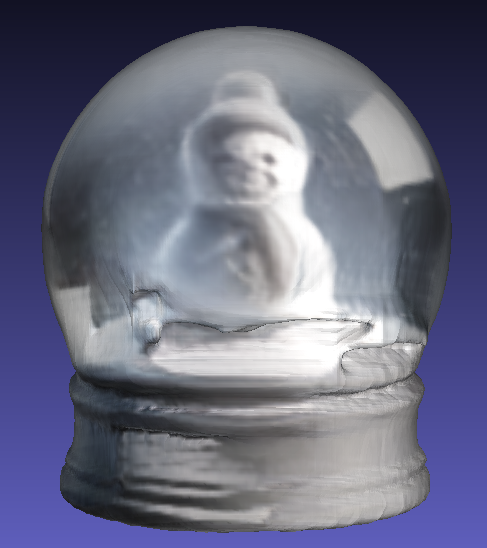
\includegraphics[width=\textwidth]{figures/subjective/wonder3d_globe_result.png}
        \caption{Wonder3D}
        \vspace{0.1cm}
    \end{subfigure}
    \begin{subfigure}[b]{0.32\textwidth}
        \centering
        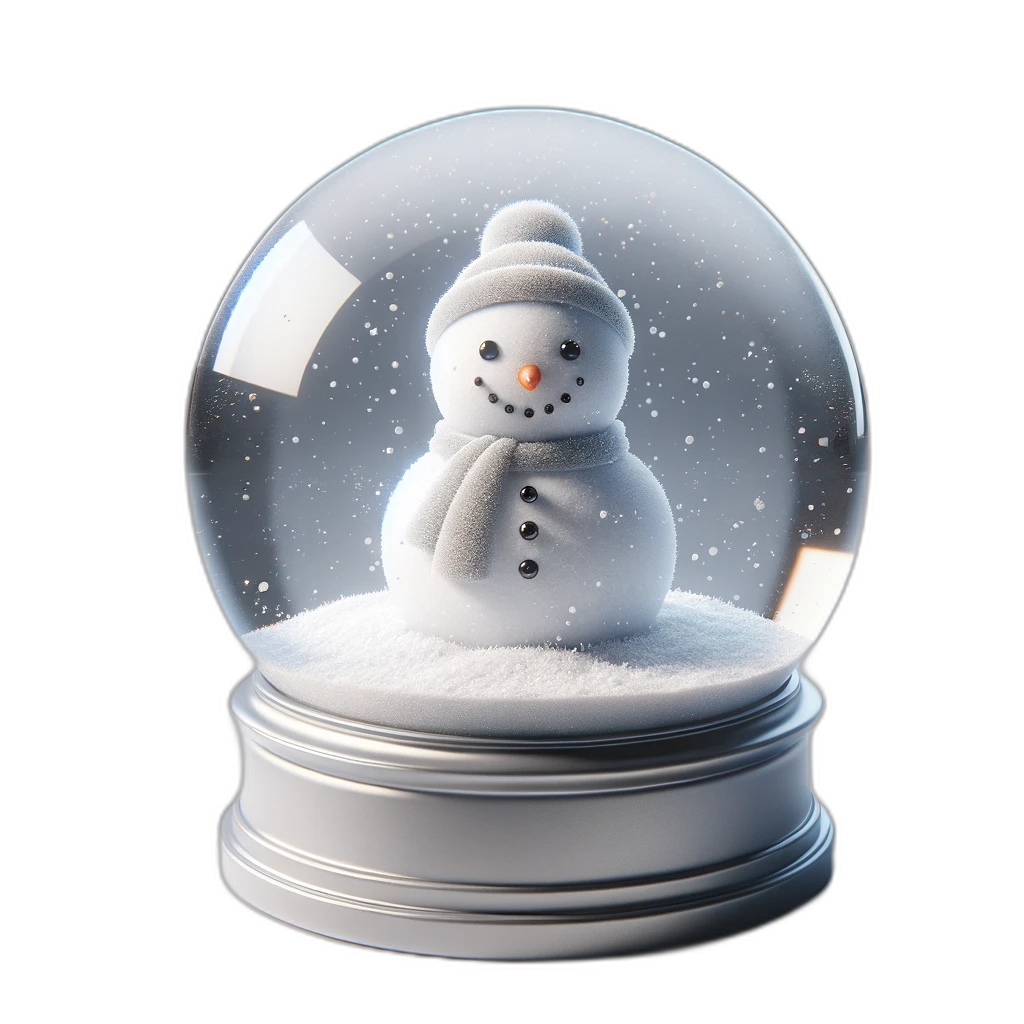
\includegraphics[width=\textwidth]{figures/input/snowGlobe.png}
        \caption{Original Image}
        \vspace{0.1cm}
    \end{subfigure}
    \caption{Using the Prompt ``a detailed rendering of a snow globe containing a snowman'' to assess transparency and difficult reflections between various methods.}~\label{fig:resultGlobe}
\end{figure}

For \textbf{Texture Realism}, an interesting phenomenon was observed across all models but Wonder3D, known as the ``Janus problem'' as named by researchers like Ben Poole from DreamFusion. This issue involves multiple faces or elements being created in a single scene, leading to duplicated details from different viewpoints. For instance, DreamFusion had a scarf on both front and back sides, while Magic3D rendered five front-view snowmen within the globe. Fantasia3D's snowman had two faces and an additional snowman printed on its back. Magic123 also duplicated front-facing snowmen. Wonder3D, benefiting from its multi-view consistency, projected only a single snowman onto the globe. However, this approach made the snowman appear as if it was printed on the glass rather than inside the globe. DreamFusion's approach, which involved using floating particles to represent glass, lost these details during the mesh conversion process. Magic3D displayed ambiguous white spots on the globe, leaving it unclear whether they represented light reflections or snow. Although the snowmen models were detailed with accessories like scarves, hats, and buttons, this detail did not extend to effectively simulating the glass of the snow globe. Fantasia3D's snowman also had detailed elements but included multiple scarfs and a flat carrot nose. Magic123 attempted to replicate reflections from the original image, yet these efforts resulted in unrealistic outcomes. Similarly, Wonder3D also had a lack of transparency, as nothing inside the globe was discernible from the back, not even the snowman's texture visible from the front. The model attempted to add reflections, but they fell short of the realism seen in the input image.

Overall, significant limitations were observed across all methods when rendering objects inside other objects, highlighting a current challenge in the field. Wonder3D, with its multi-view consistency, shows a promising approach, yet struggles like the others with achieving transparency. The interpretations of reflections from the input image led to errors, likely due to each method's unique approach to introduce lighting into the scene. This prompt resulted in the most ambiguous outcomes, highlighting major challenges and areas for future development in 3D model generation techniques


\begin{figure}[ht]
    \centering
    \small
    \begin{subfigure}[b]{0.23\textwidth}
        \centering
        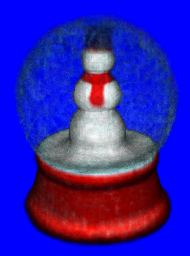
\includegraphics[width=\textwidth]{figures/subjective/dreamfusion_globe_10000_part1.png}
        \vspace{0.1cm}
        \caption{DreamFusion}
    \end{subfigure}
    \begin{subfigure}[b]{0.188\textwidth}
        \centering
        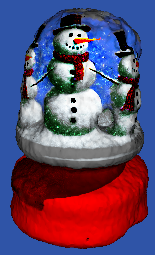
\includegraphics[width=\textwidth]{figures/subjective/59_part1.png}
        \vspace{0.1cm}
        \caption{Magic3D}
    \end{subfigure}
    \begin{subfigure}[b]{0.22\textwidth}
        \centering
        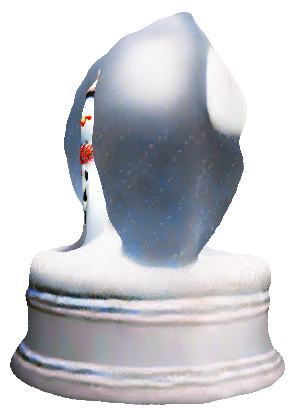
\includegraphics[width=\textwidth]{figures/subjective/it10000-3.png}
        \vspace{0.1cm}
        \caption{Magic123}
    \end{subfigure}
    \begin{subfigure}[b]{0.25\textwidth}
        \centering
        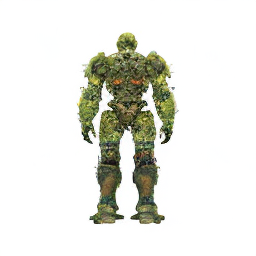
\includegraphics[width=\textwidth]{figures/subjective/rgb_000_back.png}
        \vspace{0.1cm}
        \caption{Wonder3D}
    \end{subfigure}
    \caption{Part (a): DreamFusion's attempt to create a transparent glass with multiple sliding points. Part (b) demonstrates an example of the multiple surfaces created in Magic3D. Part (c) shows the thin side view of Magic123 and part (d) provides the backside of Wonder3D and demonstrates its effectiveness in dealing with the Janus problem.}~\label{fig:dreamfusionGlobe}
\end{figure}